\documentclass[11pt]{amsart}

% -----------------------------------------------------------
% PACKAGES
\usepackage{amsmath, amsthm, amssymb}
\usepackage[T1]{fontenc}
\usepackage{lmodern}
\usepackage{hyperref}
\usepackage{enumitem}
\usepackage{setspace}
\usepackage{tikz} % CTAN: pgf

% -----------------------------------------------------------
% PAGE LAYOUT
\usepackage[margin=1in]{geometry}
\setlength{\parskip}{0.7em}
\onehalfspacing

% -----------------------------------------------------------
% TITLE INFORMATION
\title{Week 1 Reading Guide}
\author{Reading Group: \emph{The Elements of Quantitative Investing}}

% -----------------------------------------------------------
% BEGIN DOCUMENT
\begin{document}

\newtheorem{proposition}{Proposition}

\maketitle

\section{Week 0 Recap (Kickoff: May 31)}
\subsection*{Assigned Reading}
\begin{itemize}[noitemsep,left=0pt]
	\item \textbf{Chapter 2, Section 2.1:} "What Are Returns?"
	\item \emph{Background Discussion Materials:}
	      \begin{itemize}[noitemsep,left=2em]
		      \item Stylized facts of equity returns (log returns vs.\ simple returns, lower bound at $-100\%$).
		      \item Brief overview of Kalman filtering for latent‐variable estimation.
		      \item Bid–ask spread and market‐maker liquidity concepts.
	      \end{itemize}
\end{itemize}

\subsection{Key Takeaways from Section 2.1}
\begin{enumerate}[noitemsep,left=0pt]
	\item \textbf{Definition of Returns:} \\
	      \textbf{Simple/Raw/Net Returns:}
	      \[
		      R_t = \frac{P_t - P_{t-1}}{P_{t-1}},
	      \]
	      \textbf{Logarithmic Returns:}
	      \[
		      r_t = \log(1 + R_t) = \log(P_t) - \log(P_{t-1}).
	      \]
	      Logarithmic returns are additive under compounding and, for small values, are well-approximated by simple returns.
	\item \textbf{Excess Return vs.\ Total Return:}
	      Excess return is $R_t - R_{f,t}$, where $R_{f,t}$ is the risk‐free rate over period $t$. Performance metrics (Sharpe, $\alpha$) use excess returns.
	\item \textbf{Stylized Facts of Equity Returns:}
	      \begin{itemize}[noitemsep,left=2em]
		      \item Returns exhibit \emph{volatility clustering} (conditional heteroskedasticity).
		      \item Distribution is \emph{leptokurtic}: heavier tails than the normal distribution.
		      \item Autocorrelation of raw returns $\approx 0$; squared returns $r_t^2$ show persistence.
	      \end{itemize}
	\item \textbf{Kalman Filter:}
	      A method to estimate unobservable variables (e.g., latent volatility, drift) in state\textendash space models. The Kalman filter is the optimal (minimum variance) estimator under the Roll model's normally distributed (Gaussian) noise and linear state\textendash space assumptions.
	\item \textbf{Bid–Ask Spread \& Liquidity:}
	      Market makers set quotes $(\text{bid}, \text{ask})$. Spread widens during high volatility or low liquidity, affecting realized returns via transaction costs.
	\item \textbf{Clarification:} Even if simple/net returns are normally distributed, log returns are generally not exactly normal. Empirically, however, log returns often appear approximately normal over short horizons.
\end{enumerate}

\section{Week 1 Reading (June 1–7)}

\subsection{Assigned Reading}
\begin{itemize}[noitemsep,left=0pt]
	\item \textbf{Chapter 2, Sections 2.2–2.5:}
	      \begin{enumerate}[noitemsep,left=1em]
		      \item 2.2 Conditional Heteroskedastic Models
		      \item 2.3 Nonparametric Estimation of Variance
		      \item 2.4 Appendix (GARCH Stationarity and Moment Conditions)
		      \item 2.5 Exercises
	      \end{enumerate}
\end{itemize}

\subsection{Learning Objectives}
By the end of Week 1, you should be able to:
\begin{enumerate}[noitemsep,left=0pt]
	\item Derive and explain the \emph{ARCH(1)} and \emph{GARCH(1,1)} specifications.
	\item Understand why volatility clusters arise and how they're modeled parametrically.
	\item Compare \emph{parametric} (GARCH) vs.\ \emph{nonparametric} (rolling‐window or kernel) volatility estimators.
	\item Work through the appendix proofs to confirm GARCH stationarity and compute unconditional variance.
\end{enumerate}

\subsection{Section Summaries \& Discussion Questions}

\subsubsection{2.2 Conditional Heteroskedastic Models}
\paragraph{Summary:}
\begin{itemize}[noitemsep,left=0pt]
	\item ARCH(1):
	      \[
		      \varepsilon_t = h_t z_t,\quad z_t \sim \mathcal{N}(0,1)\text{ (the standard normal distribution)},
		      \quad
		      h_t^2 = \omega + \alpha \varepsilon_{t-1}^2.
	      \]
	\item GARCH(1,1):
	      \[
		      h_t^2 = \omega + \alpha \varepsilon_{t-1}^2 + \beta h_{t-1}^2.
	      \]
	\item Both capture \emph{volatility clustering}: a large value of $\varepsilon_{t-1}^2$ leads to a large value of $h_t^2$.
	\item Stationarity condition: $\alpha + \beta < 1$ for covariance\textendash stationarity.
	      \begin{proposition}
		      In a stationary GARCH(1,1) model with parameters $\omega, \alpha, \beta$ satisfying $\alpha + \beta < 1$, the unconditional variance is
		      \[
			      \operatorname{Var}(\varepsilon_t) = \frac{\omega}{1 - \alpha - \beta}.
		      \]
	      \end{proposition}
	\item \textbf{Note:} Conditional variance (volatility) can change over time based on past information, while the \emph{unconditional variance} is constant (long-run average). This distinction explains why GARCH models capture \emph{volatility clustering} and \emph{heavy tails} in returns.

	      % --- BEGIN EXPANDED CLARIFICATION ---
	      \begin{enumerate}[left=2em, label=\arabic*.]
		      \item \textbf{Conditional variance $h_t^2 = \operatorname{Var}(\varepsilon_t \mid \mathcal{F}_{t-1})$}, where $\mathcal{F}_{t-1}$ denotes the sigma-algebra generated by information available up to time $t-1$.
		            \begin{itemize}
			            \item ``Conditional'' means ``given all information up to time $t-1$'' (the $\sigma$-algebra $\mathcal{F}_{t-1}$).
			            \item In an ARCH/GARCH model this quantity is \emph{dynamic}: every time new information (the most recent squared return, past variance, etc.) arrives, the forecast for next period's variance is updated, so $h_t^2$ moves around through time.
		            \end{itemize}
		      \item \textbf{Unconditional variance $\operatorname{Var}(\varepsilon_t)$}
		            \begin{itemize}
			            \item This is the long-run, time-average variance you would get if you ignored the dating of observations and just treated every $\varepsilon_t$ as an i.i.d. draw from the same distribution.
			            \item In a stationary GARCH(1,1) with parameters $\omega,\alpha,\beta$ satisfying $\alpha+\beta<1$, that constant is
			                  \[
				                  \operatorname{Var}(\varepsilon_t)=\frac{\omega}{1-\alpha-\beta}.
			                  \]
		            \end{itemize}
		      \item \textbf{Why the distinction matters}
		            \begin{itemize}
			            \item The \emph{time-varying} $h_t^2$ explains \textbf{volatility clustering}: periods of high (or low) conditional variance persist because yesterday's large (or small) squared return feeds directly into today's variance forecast, which in turn influences tomorrow's.
			            \item Even if the shocks $z_t$ in $\varepsilon_t=h_t z_t$ are normally distributed, the fact that $h_t$ changes randomly makes the \emph{marginal} (unconditional) distribution of $\varepsilon_t$ a mixture of normals with different variances. Mixture distributions have fatter tails than any single normal component, so the model naturally produces \textbf{heavy-tailed} unconditional returns.
		            \end{itemize}
	      \end{enumerate}
	      % --- END EXPANDED CLARIFICATION ---
	\item \textbf{Volatility Persistence:} When $\alpha + \beta \approx 1$, volatility shocks decay slowly, leading to highly persistent volatility clustering.
\end{itemize}

\paragraph{Questions to Consider:}
\begin{enumerate}[noitemsep,left=0pt]
	\item Show that under GARCH(1,1), \[\mathrm{Var}(\varepsilon_t) = \frac{\omega}{1 - \alpha - \beta}.\]
	\item How does GARCH(1,1) reduce to ARCH(1) when $\beta = 0$?
	\item Explain why $\alpha + \beta$ close to 1 implies very persistent volatility shocks.
\end{enumerate}

\subsubsection{2.3 Nonparametric Estimation of Variance}
\paragraph{Summary:}
\begin{itemize}[noitemsep,left=0pt]
	\item \emph{Rolling‐window estimator} (past $m$ returns):
	      \[
		      \hat h_t^2 \;=\; \frac{1}{m - 1}\sum_{i=1}^m \bigl(R_{t-i} - \bar{R}\bigr)^2.
	      \]
	\item \emph{Kernel estimator}:
	      \[
		      \hat h_t^2 \;=\; \sum_{i=1}^T K\!\Bigl(\tfrac{i - t}{h}\Bigr)\,(R_i - \bar{R})^2.
	      \]
	\item Bias–variance tradeoff: larger window/bandwidth → smoother estimate but more lag.
\end{itemize}

\paragraph{Notation:} In these expressions, $\bar R$ denotes the sample mean of the returns. For the rolling-window estimator,
\[
	\bar R = \frac{1}{m}\sum_{i=1}^m R_{t-i},
\]
and for the kernel estimator one typically takes
\[
	\bar R = \frac{1}{T}\sum_{i=1}^T R_i,
\]
or, if using an un-normalized kernel, the weighted mean
\[
	\bar R_t = \frac{\sum_{i=1}^T K\bigl(\tfrac{i - t}{h}\bigr)\,R_i}{\sum_{i=1}^T K\bigl(\tfrac{i - t}{h}\bigr)}.
\]

\paragraph{Statistical Estimators:} More generally, let $X$ be a random variable whose distribution depends on an unknown parameter $\lambda$. An \textbf{estimator} of $\lambda$ is a sequence of functions:
\[
	\{ \hat{\lambda}_n \}_{n \geq 1}
\]
Each $\hat{\lambda}_n : \mathbb{R}^n \to \mathbb{R}$ maps $n$ observed values (realizations) of $X$, denoted $X_1, X_2, \ldots, X_n$, to an estimate of the parameter $\lambda$:
\[
	\hat{\lambda}_n = \hat{\lambda}_n(X_1, X_2, \ldots, X_n)
\]
Typically, $X_1, X_2, \ldots, X_n$ are assumed to be \textbf{independent and identically distributed (i.i.d.)} samples from the distribution of $X$.

\begin{itemize}[noitemsep,left=0pt]
	\item \textbf{Parametric estimator:} Assumes the data comes from a specific distributional family $F(\cdot; \lambda)$ with a finite-dimensional parameter vector $\lambda$. For example, GARCH models assume specific functional forms for conditional variance with parameters $(\omega, \alpha, \beta)$.
	\item \textbf{Non-parametric estimator:} Makes minimal assumptions about the underlying distribution and does not assume a specific parametric form. The rolling-window and kernel variance estimators are non-parametric because they estimate variance directly from sample data without assuming any particular distributional form for the returns.
\end{itemize}

Note that $\bar R$ itself is a \textbf{non-parametric estimator} of the expected return $\mathbb{E}[R]$, as it makes no distributional assumptions about the returns.

\paragraph{Connection to Conditional vs.\ Unconditional Variance:} The parametric/non-parametric distinction maps closely onto the conditional/unconditional variance concepts discussed in Section 2.2:
\begin{itemize}[noitemsep,left=0pt]
	\item \textbf{GARCH models} are \textbf{parametric estimators of conditional variance} $h_t^2 = \operatorname{Var}(\varepsilon_t \mid \mathcal{F}_{t-1})$. They specify exactly how today's variance depends on past information through a particular functional form with parameters $(\omega, \alpha, \beta)$.
	\item \textbf{Rolling-window and kernel estimators} are \textbf{non-parametric estimators} that estimate variance using recent data but without imposing a specific functional form for how variance depends on past information. While they do use conditioning information (recent observations), they don't assume a particular parametric structure for the conditional variance.
	\item The rolling-window estimator $\hat h_t^2 = \frac{1}{m-1}\sum_{i=1}^m (R_{t-i} - \bar{R})^2$ can be viewed as estimating a \textbf{local unconditional variance}—the variance over the recent window, treating those $m$ observations as approximately i.i.d.
\end{itemize}

\paragraph{Questions to Consider:}
\begin{enumerate}[noitemsep,left=0pt]
	\item If you choose a window of 60 days vs.\ 200 days, how does responsiveness to a volatility spike change?
	\item Under what conditions might a kernel estimate outperform a simple rolling‐window?
	\item How do you pick the bandwidth $h$ in practice?
\end{enumerate}

\subsubsection{2.4 Appendix (Stationarity \& Moments)}
\paragraph{Summary:}
\begin{itemize}[noitemsep,left=0pt]
	\item Proof that \emph{GARCH(1,1)} is covariance‐stationary if $\alpha + \beta < 1$.
	\item Calculation of $\mathbb{E}[h_t^2]$ and $\mathbb{E}[\varepsilon_t^4]$ under Gaussian $z_t$.
	\item Consequence: unconditional kurtosis $> 3$, even if $z_t$ is normal.
\end{itemize}

\paragraph{Questions to Consider:}
\begin{enumerate}[noitemsep,left=0pt]
	\item Derive the formula for $\mathbb{E}[\varepsilon_t^4]$ in a GARCH(1,1) with $z_t \sim N(0,1)$.
	\item Why does a GARCH(1,1) generate \emph{fat tails} in the unconditional distribution of $\varepsilon_t$?
	\item What happens to kurtosis as $\alpha + \beta \to 1$?
\end{enumerate}

\subsubsection{2.5 Exercises}
The exercises in the book are:
\begin{enumerate}[noitemsep,left=0pt]
	\item \textbf{ARCH(1) Moment Calculation:} Show $\mathbb{E}[\varepsilon_t^2] = \omega/(1 - \alpha)$.
	\item \textbf{GARCH(1,1) Unconditional Variance:} Verify $\mathbb{E}[h_t^2] = \omega/(1 - \alpha - \beta)$.
	\item \textbf{Simulated Return Series:} Generate 1{,}000‐point ARCH(1) series with $\omega=0.0001$, $\alpha=0.1$. Plot sample variance over time (in Python/R).
	\item \textbf{Rolling vs.\ GARCH Forecast:} On a toy daily‐return series, compute 20‐day rolling‐window variance and compare to 1‐step GARCH forecast.
\end{enumerate}

\section{Recommended Exercises for Week 1}

\begin{enumerate}[label=\arabic*.,noitemsep,left=0pt]
	\item \textbf{Derive GARCH(1,1) Unconditional Variance.}\\
	      Starting with
	      \[
		      h_t^2 = \omega + \alpha\,\varepsilon_{t-1}^2 + \beta\,h_{t-1}^2,
	      \]
	      show that
	      \[
		      \mathbb{E}[h_t^2] \;=\; \frac{\omega}{1 - \alpha - \beta}.
	      \]
	      \textit{Hint:} Use $\mathbb{E}[\varepsilon_{t-1}^2] = \mathbb{E}[h_{t-1}^2]$.

	\item Let \(h^2 = \frac{\alpha_0}{1 - \beta_1}\). Show that
	      \[
		      h_t^2 \;=\; h^2 \;+\; \alpha_1 \sum_{i=1}^\infty \beta_1^{\,i-1}\,r_{t-i}^2 \, .
	      \]


	\item \textbf{Simulate ARCH(1) and Estimate Sample Variance.}\\
	      In R/Python:
	      \begin{enumerate}[noitemsep,left=1em]
		      \item Simulate 1{,}000 draws of $\varepsilon_t = h_t\,z_t$ with $z_t \sim N(0,1)$, $\omega=10^{-4}$, $\alpha=0.2$.
		      \item Compute the sample rolling 50‐day variance of $\varepsilon_t$.
		      \item Overlay the true $h_t^2$ from the simulation.
	      \end{enumerate}
	      Write a brief discussion comparing the sample variance to the true conditional variance.

	\item \textbf{Kernel Variance Estimator.}\\
	      \begin{enumerate}[noitemsep,left=1em]
		      \item Choose a simple kernel (e.g., Gaussian) with bandwidth $h=25$.
		      \item For the same simulated ARCH series, compute
		            \[
			            \hat h_t^2 = \sum_{i=1}^{1000} K\Bigl(\tfrac{i - t}{25}\Bigr)\,\varepsilon_i^2.
		            \]
		      \item Plot this against the 50‐day rolling variance.
	      \end{enumerate}
	      Discuss how kernel smoothing might help during periods of abrupt volatility change.

	\item \textbf{Appendix Proof Checks.}\\
	      \begin{enumerate}[noitemsep,left=1em]
		      \item Reproduce the main steps in Section 2.4 to confirm that GARCH(1,1) has kurtosis $>3$.
		      \item Provide a 1–2 paragraph write‐up: Why does conditional heteroskedasticity alone generate fat‐tailed returns?
	      \end{enumerate}

	\item \textbf{Practical Question.}\\
	      \begin{enumerate}[noitemsep,left=1em]
		      \item Given a real equity return series (e.g., SPY daily returns), fit a GARCH(1,1) model.
		      \item Report estimated parameters $(\omega,\alpha,\beta)$, and check whether $\alpha + \beta < 1$.
		      \item Compare 1‐step GARCH forecast to 30‐day rolling sample variance over time.
		      \item Summarize: In which sub‐periods did GARCH outperform rolling estimation, and vice versa?
		      \item \emph{Tip:} Use \texttt{yfinance} or \texttt{pandas\_datareader} in Python to download historical SPY returns.
	      \end{enumerate}

	\item \textbf{Conditional Value-at-Risk Analysis.}\\
	      Let $(\Omega, \mathcal{F}, \mathbb{P})$ be a probability space, and let $X \in L^p(\Omega, \mathcal{F}, \mathbb{P})$ denote the negative of the portfolio return (i.e., $X = -R$) for some $1 < p < \infty$. Consider the $\alpha$-level Conditional Value-at-Risk (CVaR), defined by
	      \[
		      \mathrm{CVaR}_\alpha(X) = \frac{1}{\alpha} \int_0^\alpha \mathrm{VaR}_u(X) \, du,
	      \]
	      where
	      \[
		      \mathrm{VaR}_u(X) := \inf \{ x \in \mathbb{R} : \mathbb{P}(X \leq x) \geq u \}
	      \]
	      is the Value-at-Risk at level $u \in (0, 1)$.
	      \begin{enumerate}[noitemsep,left=1em]
		      \item Show that if $X \in L^p$ for some $p > 1$, then $\mathrm{CVaR}_\alpha(X)$ is finite for any $\alpha \in (0, 1)$.
		      \item Use Hölder's inequality to establish that
		            \[
			            \mathrm{CVaR}_\alpha(X) \leq \frac{1}{\alpha} \| X \|_p \| \mathbf{1}_{\{ X \geq \mathrm{VaR}_\alpha(X) \}} \|_q,
		            \]
		            where $\frac{1}{p} + \frac{1}{q} = 1$, and conclude that $\mathrm{CVaR}_\alpha(X) < \infty$.
	      \end{enumerate}
\end{enumerate}

\section*{Further Reading}
\begin{itemize}
	\item Engle, R. F. (1982). "Autoregressive Conditional Heteroskedasticity with Estimates of the Variance of United Kingdom Inflation." \emph{Econometrica}, 50(4), 987–1007.
	\item Bollerslev, T. (1986). "Generalized Autoregressive Conditional Heteroskedasticity." \emph{Journal of Econometrics}, 31(3), 307–327.
	\item Tsay, R. S. (2010). \emph{Analysis of Financial Time Series}. 3rd Edition, Wiley.
	\item McNeil, A. J., Frey, R., \& Embrechts, P. (2015). \emph{Quantitative Risk Management: Concepts, Techniques and Tools}. Revised Edition, Princeton University Press.
\end{itemize}

\appendix
\section{The Lebesgue Integration Layer Cake Formula}

\subsection*{The Big Picture}

In basic calculus, you learn to compute integrals using Riemann integration—think of it as adding up little rectangles under a curve. However, this method has limitations, especially when dealing with functions that have "too many" discontinuities.

Measure theory and \textbf{Lebesgue integration} provide a more flexible framework that can handle functions that Riemann integration struggles with. Instead of summing up rectangles in the horizontal direction (over the $x$-axis), Lebesgue integration "cuts" the graph of the function vertically—summing slices across \textbf{values} of the function.

\subsection*{Key Building Blocks}

\subsubsection*{1. Measure spaces}

A \textbf{measure space} is a triple $(\Omega, \mathcal{F}, \mu)$, where:
\begin{itemize}
	\item $\Omega$ is the set of outcomes (like $\mathbb{R}$ or $[0,1]$).
	\item $\mathcal{F}$ is a collection of subsets of $\Omega$ we can measure (like intervals, or more general sets).
	\item $\mu$ is a function that assigns a non-negative size (or "measure") to each set in $\mathcal{F}$.
\end{itemize}
For example, for $\mathbb{R}$, $\mu$ might be the usual \textbf{Lebesgue measure} (generalizing length, area, volume, etc.).

\subsubsection*{2. Measurable functions}

A function $f: \Omega \to \mathbb{R}$ is \textbf{measurable} if it behaves nicely with respect to these measurable sets—intuitively, if the set $\{\omega: f(\omega) > \alpha\}$ is measurable for any number $\alpha$. This ensures that we can properly "count" or "measure" the size of regions where the function exceeds a given height.

\subsubsection*{3. The Lebesgue integral}

For a \textbf{non-negative measurable function} $f: \Omega \to [0, \infty]$, the \textbf{Lebesgue integral} is defined by:
\[
	\int_\Omega f \, d\mu := \sup \left\{ \int_\Omega s \, d\mu : 0 \leq s \leq f, \; s \text{ simple} \right\},
\]
where a \textbf{simple function} is one that only takes a finite number of values—like a step function.

This is different from the Riemann integral because instead of slicing the $x$-axis (domain) into little intervals, we approximate $f$ from \textbf{below} using simple functions.

\subsection*{The Key Idea: Layer Cake Representation}

Now let's see how this approach lets us express an integral in a very different way—by slicing the graph of $f$ \textbf{horizontally}!

For a non-negative measurable function $f$, at each level $\alpha \geq 0$, consider the set of points in $\Omega$ where $f(\omega) > \alpha$:
\[
	A_\alpha := \{\omega \in \Omega : f(\omega) > \alpha\}.
\]
This is called a \textbf{superlevel set}.

Intuitively:
\begin{itemize}
	\item As $\alpha$ increases from 0 to $\infty$, $A_\alpha$ gets smaller—fewer points have function values larger than $\alpha$.
	\item At $\alpha = 0$, $A_0$ is all of $\Omega$ if $f > 0$.
	\item At very large $\alpha$, $A_\alpha$ might be empty.
\end{itemize}

\subsection*{The Layer Cake Formula}

It turns out we can \textbf{rebuild} the function $f(\omega)$ by "stacking up" the indicator functions of these level sets:
\[
	f(\omega) = \int_0^\infty \mathbf{1}_{\{\alpha < f(\omega)\}} \, d\alpha.
\]
Here, $\mathbf{1}_{\{\alpha < f(\omega)\}} = 1$ whenever $\alpha$ is below $f(\omega)$, and 0 otherwise. So for any point $\omega$, this integral simply counts the "height" of the bar up to $f(\omega)$.

\subsection*{Putting it all together: Fubini's Theorem}

We can integrate over $\omega$ and $\alpha$ in \textbf{either order} (thanks to Fubini's or Tonelli's theorem, which says you can swap the order of integration for non-negative functions):
\[
	\int_\Omega f(\omega) \, d\mu(\omega) = \int_\Omega \left( \int_0^\infty \mathbf{1}_{\{\alpha < f(\omega)\}} \, d\alpha \right) d\mu(\omega).
\]
\[
	= \int_0^\infty \left( \int_\Omega \mathbf{1}_{\{\alpha < f(\omega)\}} \, d\mu(\omega) \right) d\alpha.
\]

\subsection*{Final expression}

The inner integral counts the \textbf{measure} of the set where $f(\omega) > \alpha$:
\[
	\int_\Omega \mathbf{1}_{\{\alpha < f(\omega)\}} \, d\mu(\omega) = \mu(\{\omega : f(\omega) > \alpha\}).
\]
Thus:
\[
	\int_\Omega f(\omega) \, d\mu(\omega) = \int_0^\infty \mu(\{\omega : f(\omega) > \alpha\}) \, d\alpha.
\]

\subsection*{Intuition}

This final formula says:
\begin{itemize}
	\item The integral of the function $f$ can be seen as \textbf{adding up the areas of slices} across all possible heights $\alpha$.
	\item This is why it's called the \textbf{layer cake}: each $\alpha$ represents a horizontal "layer" of the cake, and the area of that layer is given by the measure of the set where $f(\omega) > \alpha$.
\end{itemize}

\begin{figure}[h]
	\centering
	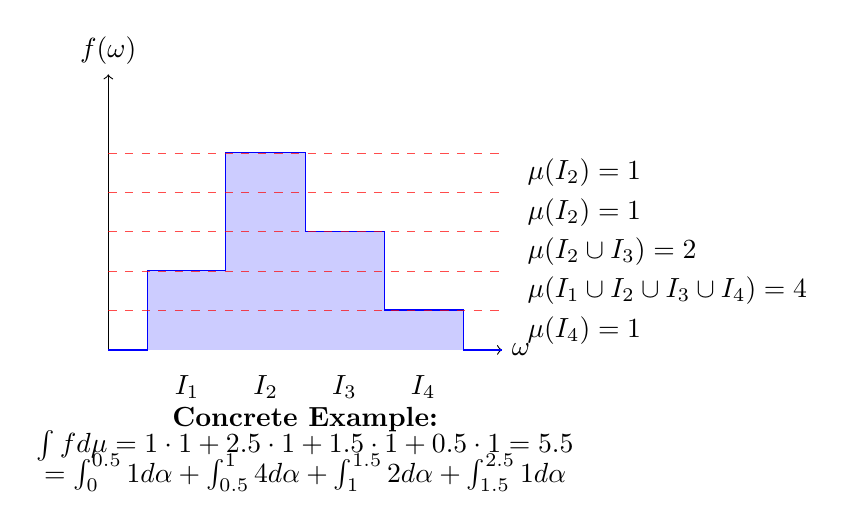
\begin{tikzpicture}[scale=1.0]
		% Simple step function example
		\draw[->] (0,0) -- (5,0) node[right] {$\omega$};
		\draw[->] (0,0) -- (0,3.5) node[above] {$f(\omega)$};

		% Draw step function
		\draw[thick, blue] (0.5,0) -- (0.5,1) -- (1.5,1) -- (1.5,2.5) -- (2.5,2.5) -- (2.5,1.5) -- (3.5,1.5) -- (3.5,0.5) -- (4.5,0.5) -- (4.5,0);
		\draw[thick, blue] (0,0) -- (0.5,0);
		\draw[thick, blue] (4.5,0) -- (5,0);

		% Fill areas
		\fill[blue!20] (0.5,0) rectangle (1.5,1);
		\fill[blue!20] (1.5,0) rectangle (2.5,2.5);
		\fill[blue!20] (2.5,0) rectangle (3.5,1.5);
		\fill[blue!20] (3.5,0) rectangle (4.5,0.5);

		% Draw horizontal grid lines for layer cake
		\foreach \y in {0.5, 1.0, 1.5, 2.0, 2.5} {
				\draw[dashed, red, opacity=0.7] (0, \y) -- (5, \y);
			}

		% Label the intervals
		\node[below] at (1, -0.2) {$I_1$};
		\node[below] at (2, -0.2) {$I_2$};
		\node[below] at (3, -0.2) {$I_3$};
		\node[below] at (4, -0.2) {$I_4$};

		% Add measure annotations
		\node[right] at (5.2, 0.25) {$\mu(I_4) = 1$};
		\node[right] at (5.2, 0.75) {$\mu(I_1 \cup I_2 \cup I_3 \cup I_4) = 4$};
		\node[right] at (5.2, 1.25) {$\mu(I_2 \cup I_3) = 2$};
		\node[right] at (5.2, 1.75) {$\mu(I_2) = 1$};
		\node[right] at (5.2, 2.25) {$\mu(I_2) = 1$};

		\node[below] at (2.5, -0.6) {\textbf{Concrete Example:}};
		\node[below] at (2.5, -0.9) {$\int f d\mu = 1 \cdot 1 + 2.5 \cdot 1 + 1.5 \cdot 1 + 0.5 \cdot 1 = 5.5$};
		\node[below] at (2.5, -1.2) {$= \int_0^{0.5} 1 d\alpha + \int_{0.5}^1 4 d\alpha + \int_1^{1.5} 2 d\alpha + \int_{1.5}^{2.5} 1 d\alpha$};
	\end{tikzpicture}
	\caption{Concrete example: For a step function, the layer cake formula sums the measures of superlevel sets at each height $\alpha$.}
\end{figure}

\subsection*{Relevance to Probability and Statistics}

The layer cake representation is particularly powerful in probability theory because it allows us to transform problems from abstract, often complex probability spaces into problems on the real line that we can handle more easily.

\paragraph{The Abstract-to-Concrete Transformation:}
In probability, we typically start with:
\begin{itemize}
	\item An abstract \textbf{probability space} $(\Omega, \mathcal{F}, \mathbb{P})$ where $\Omega$ represents all possible outcomes (e.g., all possible stock price paths, weather patterns, or experimental results).
	\item A \textbf{random variable} $X: \Omega \to \mathbb{R}$ that maps these abstract outcomes to real numbers we care about (returns, losses, temperatures, etc.).
\end{itemize}

The problem is that $\Omega$ can be incredibly complex—think of the space of all possible stock price trajectories over a year. Working directly with integrals over such spaces is often intractable.

\paragraph{The Layer Cake Solution:}
The layer cake formula transforms expectations of functions of $X$ into integrals over the real line:
\[
	\mathbb{E}[g(X)] = \int_\Omega g(X(\omega)) \, d\mathbb{P}(\omega) = \int_{-\infty}^\infty g(x) \, dF_X(x),
\]
where $F_X(x) = \mathbb{P}(X \leq x)$ is the \textbf{distribution function} of $X$. For non-negative functions $g$, this becomes:
\[
	\mathbb{E}[g(X)] = \int_0^\infty \mathbb{P}(g(X) > \alpha) \, d\alpha.
\]

\paragraph{Key Benefits:}
\begin{enumerate}[noitemsep,left=0pt]
	\item \textbf{Simplification:} We move from integration over a complex space $\Omega$ to integration over $\mathbb{R}$, which we understand well.
	\item \textbf{Distribution-free analysis:} We only need to know the \textbf{pushforward measure} $X_*\mathbb{P}$ (the distribution of $X$) rather than the details of the original probability space.
	\item \textbf{Tail behavior focus:} The formula $\int_0^\infty \mathbb{P}(X > \alpha) d\alpha$ naturally emphasizes the \textbf{tail probabilities} $\mathbb{P}(X > \alpha)$, which are crucial for risk management.
	\item \textbf{Connection to quantiles:} This perspective directly connects to \textbf{Value-at-Risk} and other quantile-based risk measures, since $\mathbb{P}(X > \alpha)$ is intimately related to the quantile function.
\end{enumerate}

\paragraph{Applications in Finance:}
For a portfolio loss $L$ (a random variable), the layer cake formula gives us:
\[
	\mathbb{E}[L] = \int_0^\infty \mathbb{P}(L > \alpha) \, d\alpha.
\]
This immediately shows that:
\begin{itemize}
	\item The expected loss is the \textbf{area under the survival function} $\alpha \mapsto \mathbb{P}(L > \alpha)$.
	\item Risk measures like \textbf{Conditional Value-at-Risk (CVaR)} can be expressed as:
	      \[
		      \text{CVaR}_\beta(L) = \frac{1}{1-\beta} \int_{\text{VaR}_\beta(L)}^\infty \mathbb{P}(L > \alpha) \, d\alpha,
	      \]
	      making the connection between tail probabilities and risk measures explicit.
	\item We can estimate or model $\mathbb{P}(L > \alpha)$ directly from data without needing to fully specify the underlying probability space of market scenarios.
\end{itemize}

In essence, the layer cake formula lets us work with the \textbf{distribution} of our random variable (which we can estimate from data) rather than the underlying \textbf{probability space} (which is typically unknown and complex).

\subsection*{Summary}
\begin{itemize}
	\item Lebesgue integration generalizes Riemann integration by "counting" the contribution of \textbf{value levels} of a function.
	\item The \textbf{layer cake representation} expresses the integral as an integral over these \textbf{superlevel sets}.
	\item This powerful viewpoint is central in probability, statistics, and risk measures, where we often want to understand the \textbf{size} of the tail of a distribution (like CVaR, Value-at-Risk, etc.).
\end{itemize}

% -----------------------------------------------------------
% END DOCUMENT
\end{document}
